\documentclass[resume]{subfiles}


\begin{document}
\section{Résolution numérique par itérations}
\begin{figure}[H]
\centering
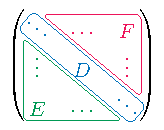
\includegraphics[scale=1,page=1]{drwg_2.pdf}
\end{figure}
\subsection{Méthode de Jacobi}
$$\vec{x}^{(k)}=D^{-1}\left(b-(A-D)\vec{x}^{(k-1)}\right)$$
$$N=D^{-1}=\text{diag}^{-1}(A)$$
\subsection{Méthode de Gauss-Seidel}
$$\vec{x}^{(k)}=(E+D)^{-1}\left(\vec{b}-F\vec{x}^{(k-1)}\right)$$
$$N=(D+E)^{-1}$$
\subsection{Méthode SOR}
$$\vec{x}^{(k+1)}=(D+\omega E)^{-1}\cdot \left(\omega \vec{b}-(\omega F+(\omega-1)D)\vec{x}^{(k)}\right)$$
\subsection{Convergence}
De manière générale on a une expression de la forme
$$\vec{x}^{(k)}=\vec{x}^{(k-1)}+\textcolor{OrangeRed}{N}\left(\vec{b}-A\vec{x}^{(k-1)}\right)$$
Avec un $\textcolor{OrangeRed}{N}$ qui se rapproche de $A^{-1}$ pour que le système soit rapide (mais sans être trop dur à calculer).\\
$$\boxed{\rho(I-NA)=\max\left(\text{valeurs propres}(I-NA)\right)}$$
$$\rho < 1\longrightarrow\text{ convergence garantie}$$
\subsubsection{Erreur}
$$e^{(k)}=\underbrace{(I-NA)}_\text{matrice d'itération}e^{(k-1)}$$
$$\abs{\abs{\vec{e}^{(k)}}}\leq \rho^{k}\abs{\abs{\vec{e}^{(0)}}}$$
Relation entre le nombre de décimales souhaitées $D$ et le nombre d'itérations $n$
$$n\geq \frac{\log_{10}(10^{-D})}{\log_{10}(\rho)}=-\frac{D}{\log_{10}(\rho)}$$
\subsection{Minimisation}
$$\boxed{\vec{r}=\vec{b}-Ax}$$
\subsubsection{Méthode $F(x)=\frac{1}{2}\abs{\abs{b-A\vec{x}}}^2_2$}
$$\boxed{\vec{d}=2A^T\vec{r}\qquad \alpha=\frac{\vec{r}^TA\vec{d}}{\vec{d}^TA^TA\vec{d}}}$$
$$\boxed{\vec{x}_{k+1}=\vec{x}_{k}+\alpha\vec{d}}$$
\subsubsection{Méthode $G(x)=\frac{1}{2}\vec{x}^TA\vec{x}-\vec{b}^T\vec{x}$}
$$\boxed{\alpha=\frac{\vec{d}^T\vec{r}}{\vec{d}^TA\vec{d}}}$$
Il existe deux méthodes
\begin{enumerate}
\item Plus grande pente (gradient). Va donner des "zig-zag"
$$\boxed{\vec{d}=\vec{r}=\vec{b}-A\vec{x}}$$
\item Gradients conjugués (réponse après $n$ itérations, avec $n$ la largeur de la matrice $A$). Le premier $\vec{d}_0$ est égal à $\vec{r}_0$ puis on le calcule avec les valeurs précédentes
$$\boxed{\vec{d}=\vec{r}+\beta_{k-1}\vec{d}_{k-1}\qquad \beta_{k-1}=\frac{\vec{r}_{k}^T\vec{r}_{k}}{\vec{r}_{k-1}^T\vec{r}_{k-1}}}$$
\end{enumerate}

\end{document}